\chapter{Visualization Layer}\label{viz-ch}

The primary function of the visualization layer is to render a spectrogram
served by the compute layer. In addition, this module is responsible for
providing a usable interface for an analyst to work with the datasets.
Minimizing latency is an important design goal since increased latency can
dramatically reduce an analyst's efficiency if they must continually wait for
the interface to respond from their queries. \\

We chose to build browser based visualizations since they allow ease of use for
an analyst, who only has to visit a webpage instead of installing any software
aside from the browser itself. Also, the analyst does not require special
hardware since the server handles the intensive storage and computations.  This
choice makes the job of visualizing interactively more difficult since the
browser is much more limited in network bandwidth and rendering capabilities
compared to a native application. (add sources to back this up, or numbers)

\section{Design}

\subsection{Interface}

The interface should provide the analyst with the ability to specify a patient
\c{mrn} to query, a \c{start\_time} and \c{end\_time} and also afford quick
navigation between time ranges. The workflow that we anticipate is that an
analyst will load a single patient file and browse subsequent time frames. Upon
reaching an interesting section, the analyst should be able to zoom in to see
further details. The interface should also give the analyst information about
the visualization, such as interactive axes. The interface should also provide
user feedback for errors, cleaning data on the client to prevent the
inadvertent issuing of queries.

\subsection{Communication}

Optimizing communication is important to avoid creating a bottleneck that can
affect latency. The point which is most likely to be a bottle neck is
deserializing the data received from the network.

\subsection{Rendering}

The client rendering must be able to efficiently render large matrices of
floating point values, on the order of several million points.  The spectrogram
visualization is created by taking the intensity $(i, j)$-th entry in the
spectrogram mapped to a rendered color in the $(i, j)$-th pixel in an image.
Some amount of data aggregation is acceptable, for example downsampling,
however the  analyst must not experience degradation of the overall data
quality. \\

\section{Implementation}

We implement the visualization layer primarily using HTML, JavaScript and CSS.
WebGl performs the client side render to take advantage of the client GPU. We
performed our tests and evaluation of the implementation with Chrome
(46.0.2490.86) and Firefox (42.0) on OSX 10.11.1 and Ubuntu 14.04. (get swang's
version of chrome/FF).

\subsection{Interface}

Figure~\ref{fig:whole-interface} shows the implementation of the interface. The
interface shows a sample of the patient \c{005} rendered between the second and
third hour of the scan. These parameters, located in the top bar, enable the
analyst to scroll to previous or next hour with a single click. The scrolling
interval defaults to 1 hour, but is configurable in the settings window. \\

\begin{figure}[h]
\begin{center}
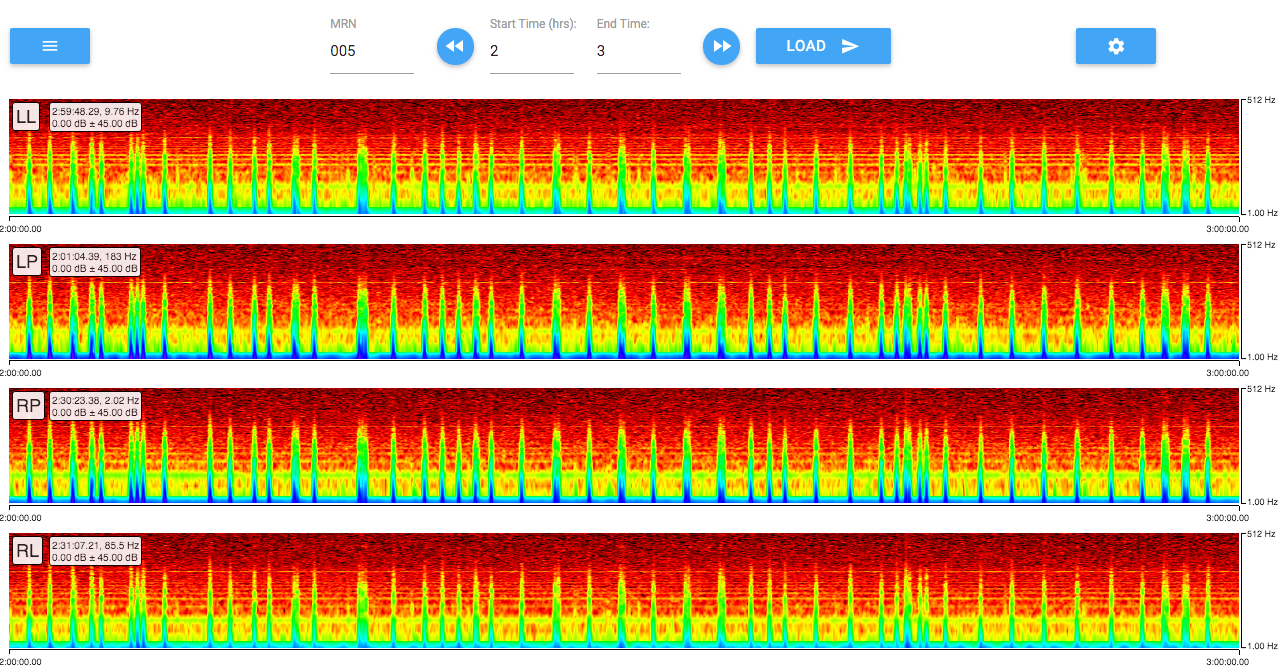
\includegraphics[scale=0.35]{./img/whole-interface.png}
\caption{Screenshot of Pinky's user interface.}
\label{fig:whole-interface}
\end{center}
\end{figure}

Clicking the the small gear on the far right of the interface opens the
settings page, Figure~\ref{fig:settings} shows the available options. The
settings page allows an analyst to change the rendering mode, time interval and
select options for interpolation and the visualization scale. In addition,
there are two keyboard shortcuts which allow an analyst to change the amplitude
scale or zoom in on the visualization. Figure~\ref{fig:zoomed-region} shows the
result of a single region when a user zoomed in. \\

\begin{figure}[h]
\begin{center}
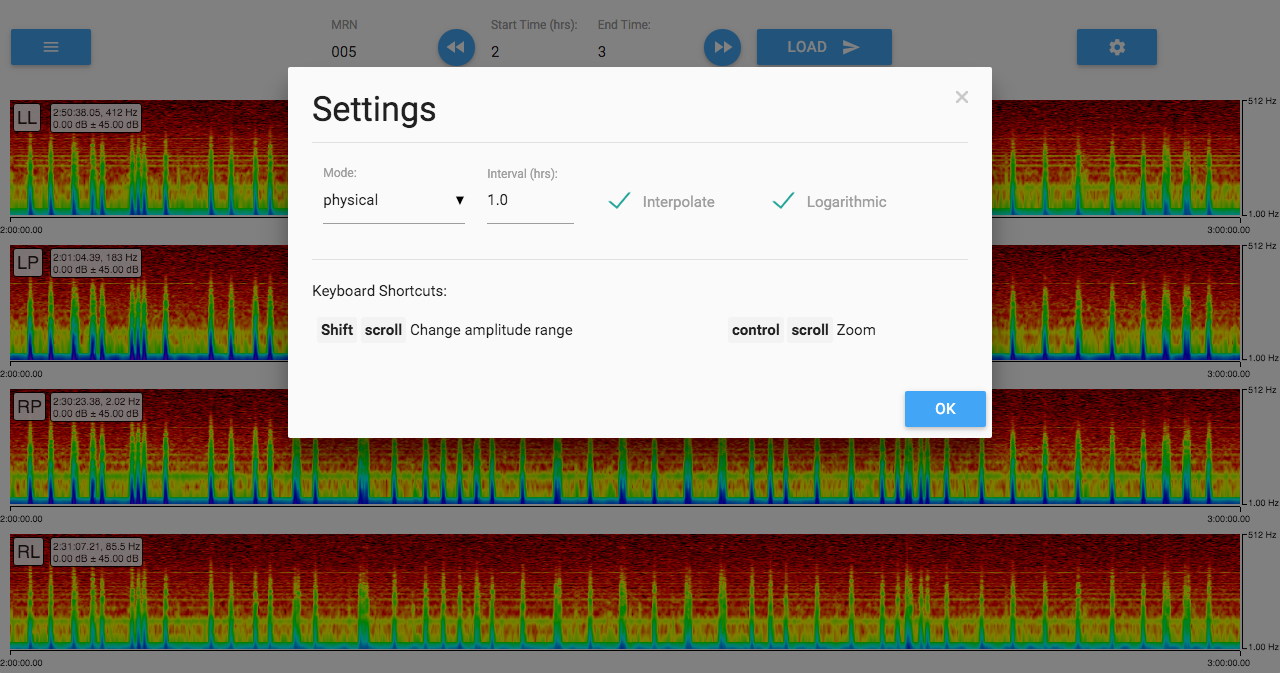
\includegraphics[scale=0.35]{./img/settings.png}
\caption{Screenshot of the settings modal.}
\label{fig:settings}
\end{center}
\end{figure}

The interface shows a spectrogram for each region of the brain, each region is
label in the upper left hand corner with \c{LL}, \c{LP}, \c{RP}, or \c{RL}.  As
Figure~\ref{fig:zoomed-region} shows, next to these labels, is a small box
containing axis information, specifying where the user's mouse currently is. In
this box the current timestamp (x-axis) and frequency (y-axis) are show. In
addition, the box shows the current amplitude value in dB and the current
amplitude viewing range. \\

\begin{figure}[h]
\begin{center}
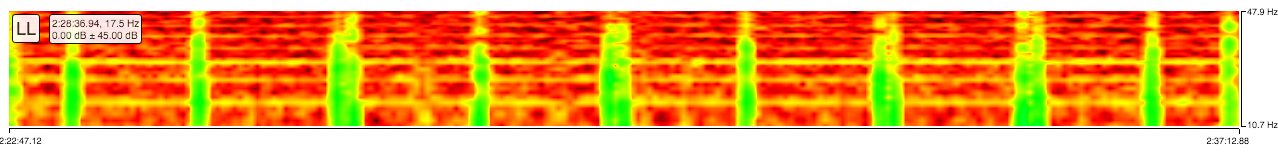
\includegraphics[scale=0.35]{./img/zoomed-region.png}
\caption{Screenshot of a zoomed spectrogram view of a single rendered region
  with dynamic axis labels.}
\label{fig:zoomed-region}
\end{center}
\end{figure}

While loading the interface blurs the spectrograms and presents a loading bar
to the user, as shown in Figure~\ref{fig:loading}. A delay between the
rendering of each region can cause confusion about the current rendered data.
Blurring a region and placing a loading bar on it clearly shows the new region
has not yet updated to the client's latest query. \\

\begin{figure}[h]
\begin{center}
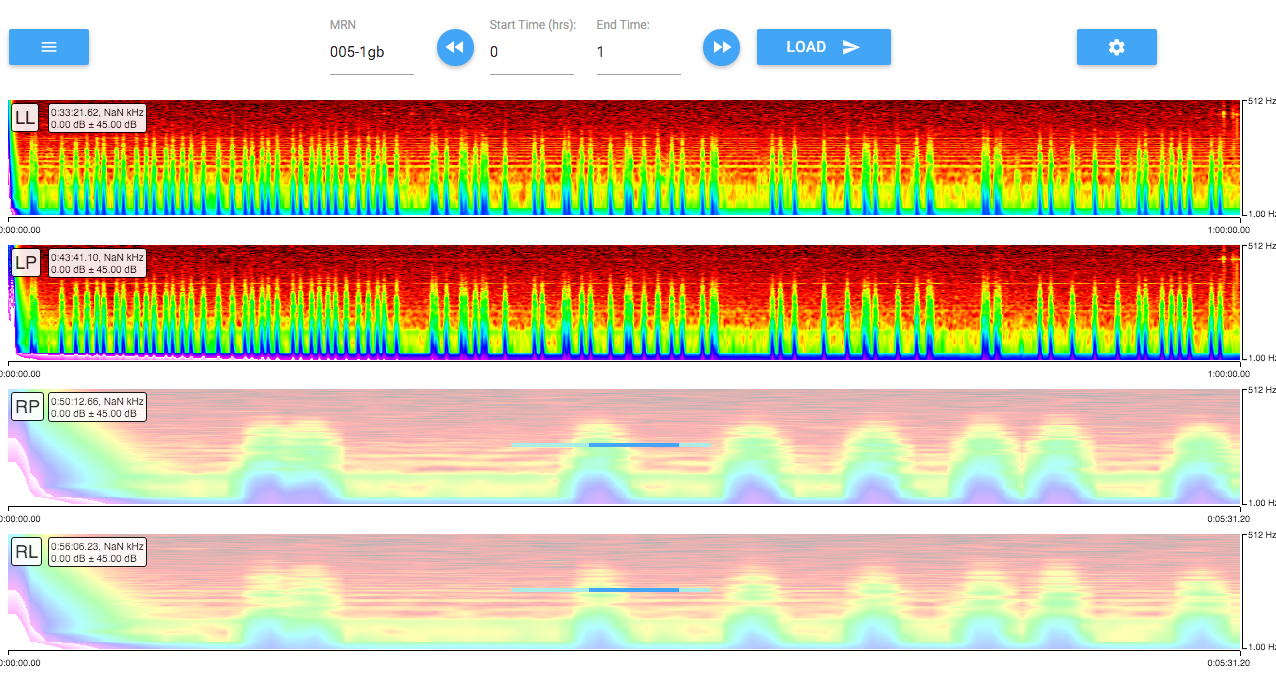
\includegraphics[scale=0.35]{./img/loading.png}
\caption{Screenshot of loading interface.}
\label{fig:loading}
\end{center}
\end{figure}

If an analyst enters an invalid \c{mrn}, the interface responds by clearing all
of the rendered spectrograms and displaying a small error message as shown in
Figure~\ref{fig:error}. An invalid \c{mrn} is simply one which the
\c{StorageBackend} does not contain an array for. This could be from a user
error or if the system is currently ingesting the array. This user interaction
is important to avoid analyst confusion when issuing an invalid query. \\

\begin{figure}[h]
\begin{center}
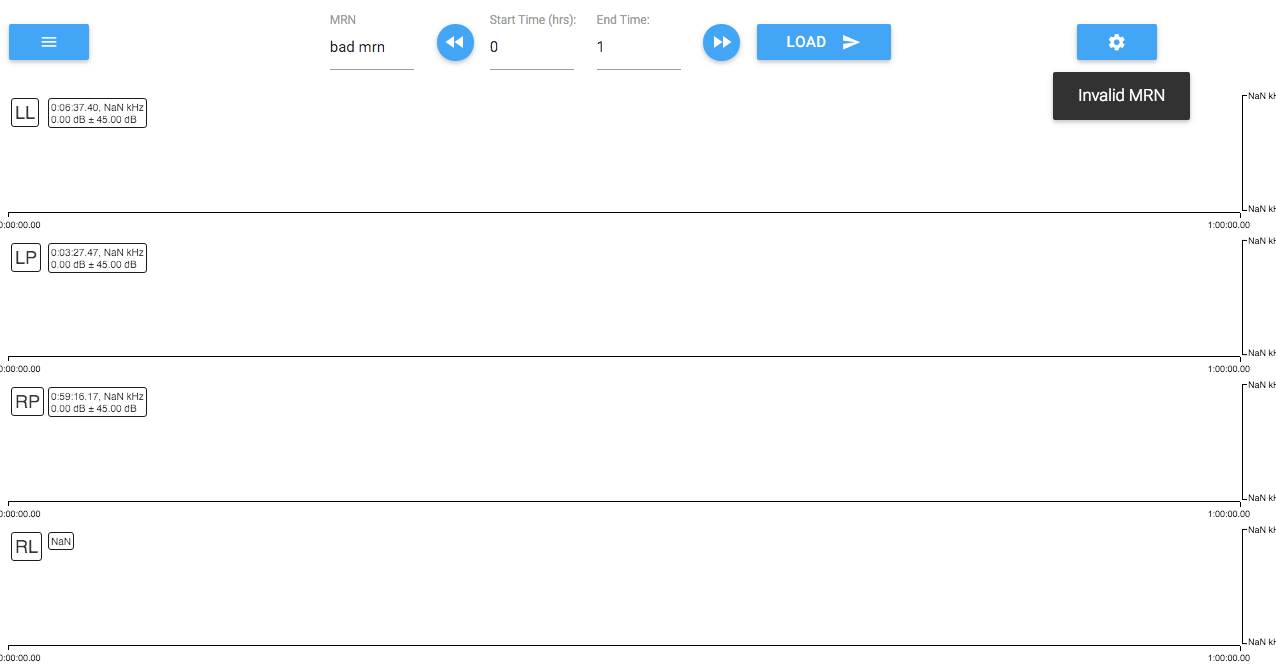
\includegraphics[scale=0.35]{./img/error.png}
\caption{Screenshot of invalid \c{mrn} error message.}
\label{fig:error}
\end{center}
\end{figure}

The materialize CSS library \cite{materialize} was used to layout the page
structure and keep a consistent style throughout the webapp.

\subsection{Communication}

A websocket communicates with the compute layer websocket server using a binary
protocol described in Section~\ref{compute-ch:implementation-ws-server}. We
send requests as JSON encoded data and receive binary responses containing the
computed spectrogram data for a given region.

We make use of the reconnecting-websocket \cite{reconnecting-websocket} library
to ensure a smooth user experience is the analyst leaves the page long enough
for the connection to close.

\subsection{Rendering}

WebGL is JavaScript API which can render interactive 2D or 3D computer graphics
without the use of any third party plugins. The initial implementation used the
open-source library WebGL-Spectrogram \cite{webgl-spectrogram}. This library
has the functionality to render the spectrogram of an audio file from a
lightweight Python websocket server. We modified this library to a more general
version to contain multiple canvases, one for each brain region, and to
communicate with the compute layer websocket server. \\

\subsection{Optimizations}

WebGL was chosen since it is much more performant than using a browser's canvas
object or rendering DOM elements directly. Each spectrogram is an array on the
order of millions of points, we would not be able to achieve the latency
required for interactivity without the GPU rendering. Development time suffers
from the use of WebGL since it is difficult to understand the programming model
without some background in graphics rendering. In addition, we use JavaScript
typed arrays to transfer the binary data from the websocket to the GPU.
JavaScript typed arrays are array-like objects providing access raw binary
data. JavaScript engines optimize these arrays giving higher performance than
the traditional JavaScript \c{Array} object.

\section{Related Work}

